\documentclass[12pt]{article}

\textwidth 17cm \textheight 25cm \evensidemargin 0cm
\oddsidemargin 0cm \topmargin -2.5cm
\parindent 0pt
%\parskip \bigskipamount

\usepackage{graphicx}
\usepackage[dutch]{babel}
\usepackage{amssymb,amsthm,amsmath}
\usepackage[utf8]{inputenc}
\usepackage{nopageno}
\usepackage{pdfpages}
\usepackage{enumerate}
\usepackage{caption}
\usepackage{wrapfig}
\usepackage{pgf,tikz}
\usepackage{color}
\usetikzlibrary{arrows}
\usetikzlibrary{patterns}
\usepackage{fancyhdr}
\pagestyle{fancy}
\usepackage[version=3]{mhchem}
\usepackage{multicol}
\usepackage{fix-cm}
\usepackage{setspace}
\usepackage{mhchem}
\usepackage{xhfill}
\usepackage{parskip}
\usepackage{cancel}
\usepackage{mdframed}
\usepackage{url}

\newcommand{\todo}[1]{{\color{red} TODO: #1}}

\newcommand{\degree}{\ensuremath{^\circ}}
\newcommand\rad{\qopname\relax o{\mathrm{rad}}}

\newcommand\ggd{\qopname\relax o{\mathrm{ggd}}}

\def\LRA{\Leftrightarrow}%\mkern40mu}

\newcommand{\zrmbox}{\framebox{\phantom{EXE}}\phantom{X}}
\newcommand{\zrm}[1]{\framebox{#1}}

% environment oefening:
% houdt een teller bij die de oefeningen nummert, probeert ook de oefening op één pagina te houden
\newcounter{noefening}
\setcounter{noefening}{0}
\newenvironment{oefening}
{
  \stepcounter{noefening}
  \pagebreak[0]
  \begin{minipage}{\textwidth}
  \vspace*{0.7cm}{\large\bf Oefening \arabic{noefening}}
}{%
  \end{minipage}
}

\usepackage{calc}

% vraag
\reversemarginpar
\newcounter{punten}
\setcounter{punten}{0}
\newcounter{nvraag}
\setcounter{nvraag}{1}
\newlength{\puntwidth}
\newlength{\boxwidth}
\newcommand{\vraag}[1]{
\settowidth{\puntwidth}{\Large{#1}}
\setlength{\boxwidth}{1.5cm}
\addtolength{\boxwidth}{-\puntwidth}
{\large\bf Vraag \arabic{nvraag} \addtocounter{nvraag}{1}}\vspace*{-0.5cm}
{\marginpar{\color{lightgray}\fbox{\parbox{1.5cm}{\vspace*{1cm}\hspace*{\boxwidth}{\Large{#1}}}}}
\vspace*{0.5cm}}
\addtocounter{punten}{#1}}

% arulefill
\newcommand\arulefill[1][]{
  \ifstrempty{#1}{
    \leavevmode{
      \xrfill[-5pt]{0.3pt}[lightgray]
      \endgraf
    }
    \vspace*{0.2cm}
  }{
    \leavevmode{
      \xrfill[-5pt]{0.3pt}[lightgray]
      \endgraf
      \vspace*{0.2cm}
    }
    \foreach \n in {1,...,#1}{
      \leavevmode{
        \xrfill[-5pt]{0.3pt}[lightgray]
        \endgraf
        \vspace*{0.2cm}
      }
    }
  }
}
% \arules{n}
\newcommand{\arules}[1]{
\mbox{}
\color{lightgray}
%\vspace*{0.05cm}
\foreach \n in {1,...,#1}{
  \vspace*{0.75cm}
  \hrule height 0.3pt\hfill
}\color{black}\vspace*{0.2cm}}

% \arule{x}
\newcommand{\arule}[1]{
\color{lightgray}{\raisebox{-0.1cm}{\rule[-0.05cm]{#1}{0.3pt}}}\color{black}
}

% \abox{y}
\newcommand{\abox}[1]{
\fbox{
\begin{minipage}{\textwidth- 4\fboxsep}
\hspace*{\textwidth}\vspace{#1}
\end{minipage}
}
}

\newcommand{\ruitjes}[1]{
\definecolor{cqcqcq}{rgb}{0.85,0.85,0.85}
\hspace*{-2.5cm}
\begin{tikzpicture}[scale=1.04,line cap=round,line join=round,>=triangle 45,x=1.0cm,y=1.0cm]
\draw [color=cqcqcq, xstep=0.5cm, ystep=0.5cm] (0,-#1) grid (20.5,0);
\end{tikzpicture}
}


\newcommand{\assenstelsel}[5][1]{
\definecolor{cqcqcq}{rgb}{0.65,0.65,0.65}
\begin{tikzpicture}[scale=#1,line cap=round,line join=round,>=triangle 45,x=1.0cm,y=1.0cm]
\draw [color=cqcqcq,dash pattern=on 1pt off 1pt, xstep=1.0cm,ystep=1.0cm] (#2,#4) grid (#3,#5);
\draw[->,color=black] (#2,0) -- (#3,0);
\draw[shift={(1,0)},color=black] (0pt,2pt) -- (0pt,-2pt) node[below] {\footnotesize $1$};
\draw[color=black] (#3.25,0.07) node [anchor=south west] { x};
\draw[->,color=black] (0,#4) -- (0,#5);
\draw[shift={(0,1)},color=black] (2pt,0pt) -- (-2pt,0pt) node[left] {\footnotesize $1$};
\draw[color=black] (0.09,#5.25) node [anchor=west] { y};
\draw[color=black] (0pt,-10pt) node[right] {\footnotesize $0$};
\end{tikzpicture}
}

\newcommand{\getallenas}[3][1]{
\definecolor{cqcqcq}{rgb}{0.65,0.65,0.65}
\begin{tikzpicture}[scale=#1,line cap=round,line join=round,>=triangle 45,x=1.0cm,y=1.0cm]
\draw [color=cqcqcq,dash pattern=on 1pt off 1pt, xstep=1.0cm,ystep=1.0cm] (#2,-0.2) grid (#3,0.2);
\draw[->,color=black] (#2.25,0) -- (#3.5,0);
\draw[shift={(0,0)},color=black] (0pt,2pt) -- (0pt,-2pt) node[below] {\footnotesize $0$};
\draw[shift={(1,0)},color=black] (0pt,2pt) -- (0pt,-2pt) node[below] {\footnotesize $1$};
\draw[color=black] (#3.25,0.07) node [anchor=south west] {$\mathbb{R}$};
\end{tikzpicture}
}

\newcommand{\visgraad}[1]{\begin{tabular}{p{0.5cm}|p{#1}}&\\\hline\\\end{tabular}}

\newcommand{\tekenschema}[2]{\begin{tabular}{p{0.5cm}|p{#1}}&\\\hline\\[#2]\end{tabular}}

% schema van Horner
\newcommand{\schemahorner}{
\begin{tabular}{p{0.5cm}|p{7cm}}
&\\[1.5cm]
\hline\\
\end{tabular}}

% geef tabular iets meer ruimte
\setlength{\tabcolsep}{14pt}
\renewcommand{\arraystretch}{1.5}

\newcommand{\toets}[3]{
\thispagestyle{plain}
\vspace*{-2.5cm}
\begin{tikzpicture}[remember picture, overlay]
    \node [shift={(15.25 cm,-1.6cm)}] {%
        \includegraphics[width=1.8cm]{/home/ppareit/kaa1415/logokaavelgem.png}%
    };%
\end{tikzpicture}

\begin{tabular}{|llc|c|}
\hline
\vspace*{-0.5cm}
&&&\\
Naam & \arule{4cm} & {\Large\bf KA AVELGEM} & \\
\vspace*{-0.75cm}
&&&\\
Klas & \arule{4cm} & {\Large\bf 20...-...-...} & \\
\hline
\vspace*{-0.75cm}
&&&\\
Toets & {\bf #2} & {\large\bf #1} & Beoordeling\\
\vspace*{-0.75cm}
&&&\\
Onderwerp & \multicolumn{2}{l|}{\bf #3} &\\
\hline
\end{tabular}
}

\newcommand{\oefeningen}[1]{

\fancyhead[LE, RO]{\vspace{0.5cm} #1}
%\thispagestyle{plain}

{\bf \Large \centering Oefeningen: #1}

}

\raggedbottom

\newcommand\dom{\qopname\relax o{\mathrm{dom}}}
\newcommand\ber{\qopname\relax o{\mathrm{ber}}}

\newcommand\mC{\qopname\relax o{\mathrm{mC}}}
\newcommand\uC{\qopname\relax o{\mathrm{{\mu}C}}}
\newcommand\C{\qopname\relax o{\mathrm{C}}}

\newcommand\W{\qopname\relax o{\mathrm{W}}}
\newcommand\kW{\qopname\relax o{\mathrm{kW}}}
\newcommand\kWh{\qopname\relax o{\mathrm{kWh}}}


\newcommand\V{\qopname\relax o{\mathrm{V}}}
\newcommand\ohm{\qopname\relax o{\mathrm{\Omega}}}
\newcommand\kohm{\qopname\relax o{\mathrm{k\Omega}}}


\newcommand\N{\qopname\relax o{\mathrm{N}}}

\newcommand\Nperkg{\qopname\relax o{\mathrm{N/kg}}}

\newcommand\Nperm{\qopname\relax o{\mathrm{N/m}}}

\newcommand\gpermol{\qopname\relax o{\mathrm{g/mol}}}


\newcommand\kgperm{\qopname\relax o{\mathrm{kg/m}}}
\newcommand\kgperdm{\qopname\relax o{\mathrm{kg/dm}}}
\newcommand\gpercm{\qopname\relax o{\mathrm{g/cm}}}
\newcommand\gperml{\qopname\relax o{\mathrm{g/ml}}}


\newcommand{\mA}{\;\mbox{mA}}
\newcommand{\A}{\;\mbox{A}}
\newcommand{\MA}{\;\mbox{MA}}

\newcommand{\us}{\;\mu\mbox{s}}
\newcommand\s{\qopname\relax o{\mathrm{s}}}

\newcommand\h{\qopname\relax o{\mathrm{h}}}

\newcommand{\mpers}{\;\mbox{m/s}}
\newcommand{\kmperh}{\;\mbox{km/h}}
\newcommand{\kmpermin}{\;\mbox{km/min}}
\newcommand{\kmpers}{\;\mbox{km/s}}

\newcommand{\mph}{\;\mbox{mph}}

\newcommand{\Hz}{\;\mbox{Hz}}

\newcommand\Gm{\qopname\relax o{\mathrm{Gm}}}
\newcommand\Mm{\qopname\relax o{\mathrm{Mm}}}
\newcommand\km{\qopname\relax o{\mathrm{km}}}
\newcommand\hm{\qopname\relax o{\mathrm{hm}}}
\newcommand\dam{\qopname\relax o{\mathrm{dam}}}
\newcommand\m{\qopname\relax o{\mathrm{m}}}
\newcommand\dm{\qopname\relax o{\mathrm{dm}}}
\newcommand\cm{\qopname\relax o{\mathrm{cm}}}
\newcommand\mm{\qopname\relax o{\mathrm{mm}}}
\newcommand\um{\qopname\relax o{\mathrm{{\mu}m}}}
\newcommand\nm{\qopname\relax o{\mathrm{nm}}}


\newcommand\Gg{\qopname\relax o{\mathrm{Gg}}}
\newcommand\Mg{\qopname\relax o{\mathrm{Mg}}}
\newcommand\kg{\qopname\relax o{\mathrm{kg}}}
\newcommand\hg{\qopname\relax o{\mathrm{hg}}}
\renewcommand\dag{\qopname\relax o{\mathrm{dag}}}
\newcommand\g{\qopname\relax o{\mathrm{g}}}
\newcommand\dg{\qopname\relax o{\mathrm{dg}}}
\newcommand\cg{\qopname\relax o{\mathrm{cg}}}
\newcommand\mg{\qopname\relax o{\mathrm{mg}}}
\newcommand\ug{\qopname\relax o{\mathrm{{\mu}g}}}
\renewcommand\ng{\qopname\relax o{\mathrm{ng}}}

\newcommand\ton{\qopname\relax o{\mathrm{ton}}}

\newcommand\Gl{\qopname\relax o{\mathrm{Gl}}}
\newcommand\Ml{\qopname\relax o{\mathrm{Ml}}}
\newcommand\kl{\qopname\relax o{\mathrm{kl}}}
\newcommand\hl{\qopname\relax o{\mathrm{hl}}}
\newcommand\dal{\qopname\relax o{\mathrm{dal}}}
\renewcommand\l{\qopname\relax o{\mathrm{l}}}
\newcommand\dl{\qopname\relax o{\mathrm{dl}}}
\newcommand\cl{\qopname\relax o{\mathrm{cl}}}
\newcommand\ml{\qopname\relax o{\mathrm{ml}}}
\newcommand\ul{\qopname\relax o{\mathrm{{\mu}l}}}
\newcommand\nl{\qopname\relax o{\mathrm{nl}}}

\newcommand\MJ{\qopname\relax o{\mathrm{MJ}}}
\newcommand\kJ{\qopname\relax o{\mathrm{kJ}}}
\newcommand\J{\qopname\relax o{\mathrm{J}}}

\newcommand\T{\qopname\relax o{\mathrm{T}}}
\newcommand\uT{\qopname\relax o{\mathrm{{\mu}T}}}

\newcommand\grC{\qopname\relax o{\mathrm{{\degree}C}}}

\newcommand\K{\qopname\relax o{\mathrm{K}}}
\newcommand\calperK{\qopname\relax o{\mathrm{cal/K}}}

\newcommand\hPa{\qopname\relax o{\mathrm{hPa}}}
\newcommand\Pa{\qopname\relax o{\mathrm{Pa}}}

\newcommand\dB{\qopname\relax o{\mathrm{dB}}}

\newcommand{\EE}[1]{\cdot 10^{#1}}

\onehalfspacing

%\singlespacing
%\onehalfspacing
%\doublespacing

%\setlength{\headsep}{0cm}

\newenvironment{exlist}[1] %
{ \begin{multicols}{#1}
  \begin{enumerate}[(a)]
    \setlength{\itemsep}{0.8em} }
{ \end{enumerate}
  \end{multicols} }




\begin{document}

\thispagestyle{empty}
\begin{center}
  \begin{mdframed}
  \centering
  \fontsize{35}{70}\selectfont Veeltermfuncties
  \end{mdframed}
  \vfill
  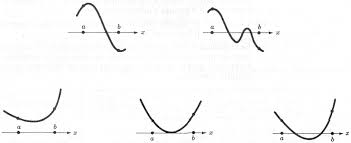
\includegraphics[width=0.8\textwidth]{veeltermen}
  \vfill
\end{center}
%\vfill
\vspace*{-2cm}
\subsection*{Doelstellingen}
{\singlespacing

Je kan \hfill  {\scriptsize(LP 2005/069, LI 1.2, ET10,11,12,13)}
\begin{itemize}
  \item vergelijkingen van de eerste en tweede graad in één onbekende oplossen.
  \item veeltermvergelijkingen van graad hoger dan 2 oplossen met behulp van ICT.
  \item aan de hand van het functievoorschrift
        \begin{itemize}
          \item een tabel,
          \item het domein,
          \item de nulwaarden,
          \item het tekenverloop,
          \item de grafiek
        \end{itemize}
        bepalen van veeltermfuncties van de eerste en tweede graad;
  \item aan de hand van de grafiek het stijgen/dalen en de extrema van veeltermfuncties van de eerste en tweede graad bepalen;
  \item met behulp van ICT de tabel en de grafiek lezen(domein, nulwaarden, tekenverloop, stijgen/dalen, extrema) van veeltermfuncties van graad hoger dan twee.
  \item veranderingen beschrijven en vergelijken met behulp van differentiequotiënten.
  \item een vraagstuk of probleem, dat aanleiding geeft tot een veeltermfunctie, wiskundig formuleren;
  \item de door het functioneel verband bekomen vergelijking oplossen;
  \item de gevonden oplossing terug vertalen naar de oplossing van het oorspronkelijke vraagstuk of probleem;
  \item problemen met gegeven functioneel verband oplossen en deze oplossing interpreteren.
\end{itemize}

}
\thispagestyle{empty}
\mbox{}
\newpage
\clearpage
\thispagestyle{empty}
\mbox{}
\newpage
\clearpage
\pagenumbering{arabic} 


\fancyhead[RO,LE]{Reële Functies}
\fancyhead[RE,LO]{}

\onehalfspacing

\section{Veeltermfuncties}

\subsection{Veeltermvergelijkingen}

\begin{oefening}
Beschouw de vergelijking
$$x^3-6x^2+5x+12=0\;.$$
\begin{enumerate}[(a)]
  \item Onderzoek of de gehele getallen van -3 tot 3 aan deze vergelijking voldoen.
  \item Zijn er nog andere getallen die aan deze vergelijking voldoen?
\end{enumerate}

\subsection{Vergelijkingen van de eerste graad}

\end{oefening}
\begin{oefening}
Los de volgende vergelijkingen van de eerste graad op in $\mathbb{R}$
\begin{enumerate}[(a)]
  \itemsep0.7em
  \item $4x-8=0$
  \item $3x+9=0$
  \item $-3x+9=0$
  \item $2(x+6)=4-(x+7)$
  \item $x - \dfrac{x-2}{3} = 4$
  \item $2(x-3)+7=5-(2-x)$
  \item $(x+1)^2-2=x(x-3)-(1-2x)$
  \item $\dfrac{3+2x}{4}-\dfrac{4x-5}{5}=\dfrac{21-6x}{6}$
  \item $\dfrac{4x}{3}-\left(\dfrac{3}{2}-\dfrac{x}{4}\right)=x+4\left(\dfrac{2x}{3}-1\right)$
  \item $\dfrac{3(x-1)}{5}-\dfrac{2(1-4x)}{7}=x+\dfrac{x+1}{5}$
  \item $\dfrac{5x}{8}-\dfrac{x-\frac{5}{2}}{4}=1$
  \item $\dfrac{x}{5}+\dfrac{x}{2}=-7$
  \item $\dfrac{3-x}{4}-\dfrac{x-2}{3}=\dfrac{x}{2}-\dfrac{4x+1}{12}$
\end{enumerate}
\end{oefening}

\begin{oefening}
Los de volgende vergelijkingen van de tweede graad op in $\mathbb{R}$
\begin{enumerate}[(a)]
  \itemsep0.7em
  \item $2x^2-4x-6=0$
  \item $5x(x-2)=x(3x-4)-5$
  \item $\frac{2}{3}x^2+5x+1=0$
  \item $80x^2+8x=15$
  \item $80x^2+15=-8x$
  \item $(3-x)(3+x)=(x-4)^2$
  \item $(x-2)^2=x^2-4$
  \item $(3x+2)(3x-2)+6x+5=0$
  \item $x+1=(x+1)(x-1)$
  \item $4x^2-20x+25=0$
  \item $3x^2+5=0$
  \item $x=x^2$
  \item $2\left(7x+32\right)=(3x+8)^2$
  \item $11x+13=2x^2$
  \item $x\left(x+3\right)+2\left(5+2x\right)=0$
  \item $x^2+2x-8=0$
  \item $(x+3)^2=16$
  \item $9x^2+30x+25=0$
  \item $10x^2+7x-3=0$
  \item $x^2=x+1$
  \item $37x^2+13x-50=0$
  \item $3x(3x+10)+5=-20$
  \item $x^2=3x-18$
\end{enumerate}
\end{oefening}

\begin{oefening}
Maak gebruik van Geogebra om de volgende vergelijkingen op te lossen in $\mathbb{R}$
\begin{enumerate}[(a)]
  \itemsep0.7em
  \item $-5x+4=0$
  \item $2(x+6)=4-(x+7)$
  \item $2x^2-4x-6=0$
  \item $5x(x-2)=x(3x-4)-5$
  \item $3x^3+x^2-8x+4=0$
  \item $x^3+6x^2-x-30=0$
  \item $x^3-3x^2+4=0$
  \item $-4(x-5)=3(2x+1)$
  \item $(x+\sqrt{5})(x^2+2x-8)=0$
  \item $5x^2+3x-4=0$
\end{enumerate}
\end{oefening}


\newpage

\subsection{Veeltermfuncties}


\begin{oefening}
Maak voor de volgende functies een tabel en een grafiek. Noteer aan de hand van de grafiek het domein, het bereik, de nulwaarde(n), het tekenverloop, het stijgen en dalen, de extreme waarde (minima en maxima) en de symmetrieën.
\end{oefening}
\begin{enumerate}[(a)]
  \item $f(x)=\frac{2}{3}x+2$
  \item $f(x)=0.5x^2-x-1.5$
  \item $f(x)=-\frac{3}{4}x^2+3x$
  \item $f(x)=3x^2-0.5x^3$
\end{enumerate}

\newpage

\begin{oefening}
Met Geogebra werd de grafiek van de functie met functievoorschrift
$$f(x)=x^5-5x^3+4x$$ gegenereerd. Lees aan de hand van de grafiek het domein, de nulwaarden en de extrema af. Bepaal het tekenverloop, het stijgen en dalen en de symmetrieën van de functie.
\end{oefening}
\begin{center}
\definecolor{cqcqcq}{rgb}{0.75,0.75,0.75}
\begin{tikzpicture}[line cap=round,line join=round,>=triangle 45,x=1.0cm,y=1.0cm]
\draw [color=cqcqcq,dash pattern=on 2pt off 2pt, xstep=1.0cm,ystep=1.0cm] (-7.22,-6.82) grid (8.13,6.66);
\draw[->,color=black] (-7.22,0) -- (8.13,0);
\foreach \x in {-7,-6,-5,-4,-3,-2,-1,1,2,3,4,5,6,7,8}
\draw[shift={(\x,0)},color=black] (0pt,2pt) -- (0pt,-2pt) node[below] {\footnotesize $\x$};
\draw[color=black] (7.87,0.07) node [anchor=south west] { x};
\draw[->,color=black] (0,-6.82) -- (0,6.66);
\foreach \y in {-6,-5,-4,-3,-2,-1,1,2,3,4,5,6}
\draw[shift={(0,\y)},color=black] (2pt,0pt) -- (-2pt,0pt) node[left] {\footnotesize $\y$};
\draw[color=black] (0.08,6.33) node [anchor=west] { y};
\draw[color=black] (0pt,-10pt) node[right] {\footnotesize $0$};
\clip(-7.22,-6.82) rectangle (8.13,6.66);
\draw[line width=1.6pt, smooth,samples=100,domain=-2.2:2.2] plot(\x,{(\x)^5-5*(\x)^3+4*(\x)});
\end{tikzpicture}
\end{center}

\begin{oefening}
Teken de grafiek van de eerstegraadsfunctie die als nulwaarde $x=3$ heeft en die de $y$-as snijdt in het punt $(0,-6)$. Kan je het functievoorschrift vinden voor deze functie?
\end{oefening}

\begin{oefening}
Teken de grafiek van de tweedegraadsfunctie die de nulwaarden $x=-1$ en $x=3$ heeft en die als top het punt $(1,4)$ heeft. Je weet verder nog dat de grafiek de $y$-as snijdt in het punt $(0,3)$. Kan je het functievoorschrift vinden voor deze functie?
\end{oefening}

\newpage
\subsection{Toepassingen}

\begin{oefening}
\begin{wrapfigure}[6]{r}{4cm}
\vspace*{-1.75cm}
\begin{center}
  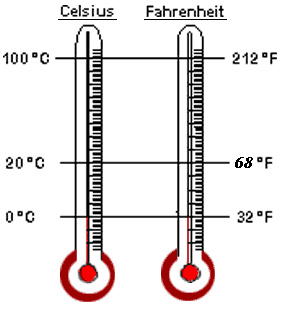
\includegraphics[width=4cm]{CelsiusFahrenheitThermo}
\end{center}
\end{wrapfigure}
Het verband tussen het aantal graden Fahrenheit ($F$) en het aantal graden Celsius ($C$) wordt gegeven door$$F=1.8C+32\;.$$
Bij welke temperatuur $T$ is het zowel $T$ graden Celsius als $T$ graden Fahrenheit?
\end{oefening}

\begin{oefening}
Na de bereiding van een ovenschotel op een temperatuur van $180\degree C$ wordt de oven afgezet. Telkens wanneer er $5$ minuten voorbij zijn, is de temperatuur $10\degree C$ gezakt.
\begin{enumerate}[(a)]
  \item Bepaal de oventemperatuur een half uur na het uitzetten. (Tip: stel een functiewaardentabel op.)
  \item Met welke formule kun je de oventemperatuur $T$ berekenen op een willekeurig tijdstip $t$? (Maw. stel een functievoorschrift op.)
  \item Teken de grafiek. Houd er rekening mee dat, als de temperatuur tot $20\degree C$ is gedaald, het afkoelingsproces stopt.
\end{enumerate}
\end{oefening}

\begin{oefening}
Je bent lid van een comité dat een spaghetti-avond organiseert ten voordele van je sportclub. Je doel is om voor 1500 euro spaghetti-tickets te verkopen. Hoeveel moet je vragen voor een ticket voor een volwassene en hoeveel voor een ticket voor een een kind, rekening houdend met de aanwezigheid van 200 volwassenen en 100 kinderen vorig jaar.

Dit probleem heeft vele oplossingen. Je zou bijvoorbeeld 6 euro per volwassene en 3 euro per kind kunnen vragen of 4 euro per volwassene en 7 euro per kind of \ldots.
\begin{enumerate}[(a)]
  \item Noteer een functievoorschrift voor dit probleem.
  \item Het comité beslist aan alle volwassenen $5.5$ euro te vragen. Hoeveel zal dan voor elk kind gevraagd worden?
\end{enumerate}
\end{oefening}

\begin{oefening}
Een vijver heeft de vorm van een cilinder. De diameter bedraagt $2$ meter en hij is $80$ cm met water gevuld. Door verdamping daalt het waterpeil dagelijks gemiddeld met $0.3$ cm. Na hoeveel dagen is de vijver leeg?
\end{oefening}

\begin{oefening}
Je gooit een bal van het dak van de hoogste verdieping van een hoog gebouw ($60$ meter hoog). Je kunt de hoogte van de vallende bal weergeven door het voorschrift:
$$h=60-\frac{1}{2}gt^2$$
waarbij:
\begin{itemize}
  \item $h$ de hoogte uitgedrukt in meters is,
  \item $g=9.81 \;m/s^2$ de valversnelling is,
  \item $t$ het tijdstip uitgedrukt in seconden is.
\end{itemize}
\begin{enumerate}[(a)]
  \item Maak een tabel en een grafiek van de val.
  \item Na hoeveel seconden bereikt de bal de grond (rond af op een honderdste van een seconde)?
\end{enumerate}
\end{oefening}

\begin{oefening}
\begin{wrapfigure}[4]{l}{3cm}
\vspace*{-1.2cm}
\begin{center}
  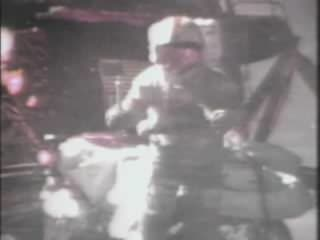
\includegraphics[width=3cm]{davidscott}
\end{center}
\end{wrapfigure}

In 1971 demonstreerde astronaut Davit Scott dat op de maan een veer en een hamer even snel vallen, omdat er op de maan geen atmosfeer en dus geen luchtweerstand is. Om de maan is de valversnelling $g=1.65 \;m/s^2$.

\begin{enumerate}[(a)]
  \item Je laat op de maan een hamer en een veer vallen vanaf $5$ meter. Na hoeveel seconden bereiken ze de maanbodem (rond opnieuw af tot op een honderdste van een seconde)?
  \item Wanneer bereikt de hamer de aardbodem bij dezelfde proef?
\end{enumerate}
\end{oefening}

\begin{oefening}
Is het mogelijk dat een rechthoek een omtrek heeft van $52$ cm en een oppervlakte van $148.75$ cm$^2$? Verklaar.
\end{oefening}

\begin{oefening}
Twee schepen verlaten tegelijkertijd de haven van Zeebrugge. Het schip 'De Regenboog' vaart naar het westen en het schip 'De Viking' vaart naar het noorden. Na verloop van tijd bevinden ze zich op $270$ km afstand van elkaar. 'De Viking' heeft $50$ km meer gevaren dan 'De Regenboog'.
\begin{enumerate}[(a)]
  \item Maak een schets van de situatie.
  \item Bereken van elk schip de afgelegde afstand tot de haven van Zeebrugge (rond af op 1 $km$).
\end{enumerate}
\begin{center}
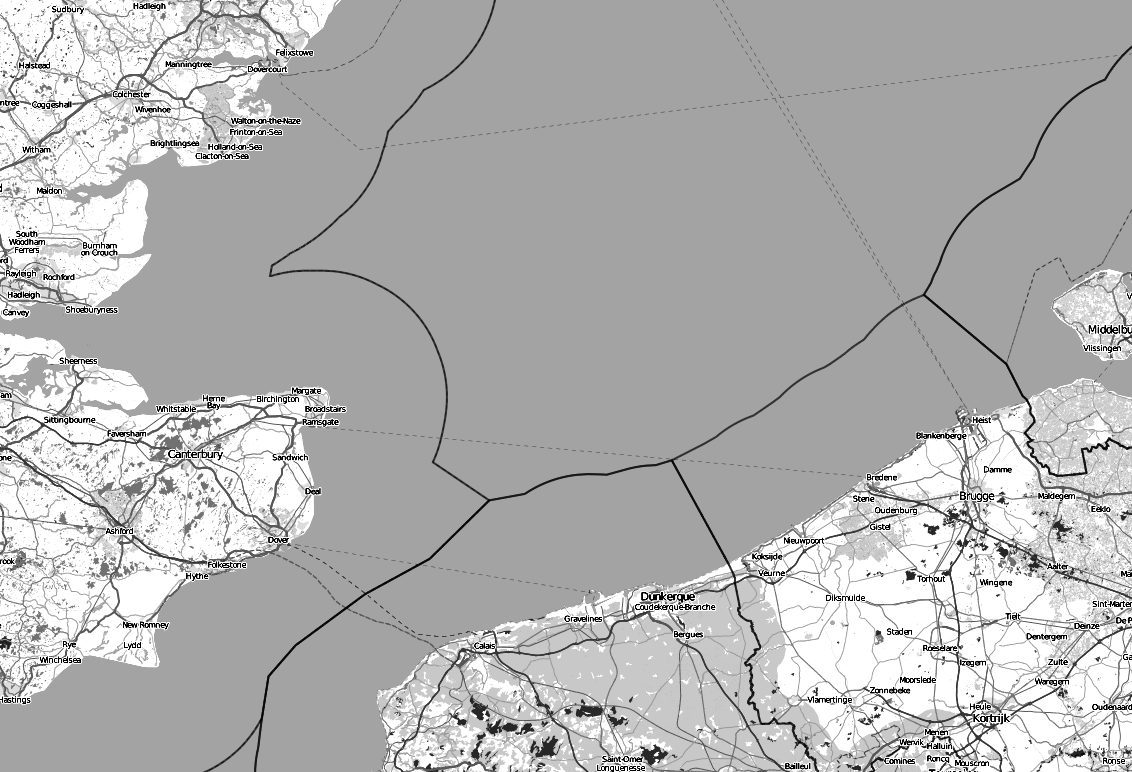
\includegraphics[width=\textwidth]{zeebrugge}
\end{center}
\end{oefening}



\end{document}
